\newpage
\chapter{Применение методов обучения с подкреплением в задаче разработки регуляторов для сложных систем управления} \label{ch3}

% не рекомендуется использовать отдельную section <<введение>> после лета 2020 года
%\section{Введение} \label{ch3:intro}

В данной главе будут рассмотрены практические примеры применения алгоритмов RL для задачи управления обратного маятника и сложных систем, которые описываются моделями типа <<хищник-жертва>>: развитие опухоли, производство пенициллина. 
	
\section{Задача управления обратным маятником} \label{ch3:sec1}
Рассмотрим следующую математическую модель перевернутого маятника:
%
\begin{equation*}
%\label{pendulum}
\ddot \vartheta_t = -0.01 \dot \vartheta_t + 9.8 \sin \vartheta_t - U_t \cos \vartheta_t
\end{equation*}
%
где $\vartheta_t \in \mathbb{R}$ -- угол наклона маятника; $U_t \in \mathcal{U}$ -- крутящий момент приложенный к маятнику в момент времени $t$. Параметры модели маятника: \(m\) = 1 кг; \(l\) = 1 м; \(g\) = 9.8 м/с²; \(\mu\) = 0.01;
Пространство действий может быть задано как $\mathcal{U}=[-u_{max},u_{max}] \subset \mathbb{R}$, при ограничении $u_{max} = 5$ Н $\cdot$ м. Динамика системы может быть представлена как:
%
\begin{equation*}
	f_d(x) = 
	\begin{bmatrix}
		x_2 \\
		9.8 \sin x_1 - 0.01x_2
	\end{bmatrix}
	, F_c(x)=
	\begin{bmatrix}
		0\\
		-\cos x_1
	\end{bmatrix}
\end{equation*}
%
где $x = [x_1, x_2]^T \in \mathbb{R}^2$. При моделировании устанавливаем коэффициент дисконтирования равный $\gamma = 0.1$ и шаг по времени \(\Delta t = 10\) мс.

Цель управления -- качнуть вверх и, в конечном итоге, установить маятник в вертикальное положение $2\pi k$ для некоторого $k \in \mathbb{Z}$ при ограничении крутящего момента $|U_t| \leq u_{max}$. 

Нахождение оценки политики $V_i$ на каждой итерации $i$ производится аппроксимируя линейную функцию:
%
\begin{equation*}
V_i(x) \approx V(x; \theta_i) = \theta^T_i \phi(x),
\end{equation*}
где $\theta_i \in \mathbb{R}^L$ - веса и $\phi(x)$ признаки с $L=121$ 

Поскольку для шага улучшения политики требуется дифференцируемая функция, выбрана радиально-базисные функция в качестве признаков $\phi(x)$, следовательно, $j$-я компонента вектора признаков $\phi(x)$ задается как:
%
\begin{equation*}
	\phi_j(x) = \exp(-(x - c_j)^T \Sigma^{-1}(x-c_j))
\end{equation*}
%
где $\Sigma^{-1}$ -- весовая матрица, а $c_j$ - центральные точки радиально базисных функций.

Рассматривается функция вознаграждения $r$, заданная формулами:
\begin{equation*}
r(x,u) = \mathfrak r(x) - \mathfrak c(u)
\end{equation*}
где $\mathfrak r(x)$ и $\mathfrak c(u)$ для непрерывного управления, применяя алгоритм DPI, имеют следующий вид:
	\begin{equation*}
	\begin{split}
	\mathfrak r(x) &= \cos x_1\\
	\mathfrak c(u) &= \lim_{v->u} \int_0^v {(s^T)^{-1}}(\mathfrak u) \cdot \text{Г} du\\
	s(\mathfrak u) &= u_{\max} \tanh(\mathfrak u/u_{\max})\\
	\end{split}
	\end{equation*}

При этом функция $s$ задает ограничения модели. Г - положительно определенная матрица.
%
Для решения задачи управления, был использован следующий метод обучения с подкреплением: \textit{Дифференциальная оценка по стратегиям} (англ. Differential Policy Iteration, DPI) ~---
алгоритм оценивает и улучшает стратегию, начиная от начальной допустимой стратегии \( \pi_0 \) и до тех пор, пока оценка и стратегия не сойдутся. На этапе оценки стратегии производится расчет дифференциального уравнения Беллмана, чтобы получить функцию стоимости \(v_i = v_{\pi_{i-1}}\) для последней стратегии \( \pi_{i - 1} \):
\begin{equation}
\alpha \cdot v_i(x) = h(x, \pi_{i-1}(x), \nabla v_i(x))   \forall x \in X
\end{equation}
Далее рассчитанное значение \(v_i\) используется в улучшении стратегии, то есть для получения следующей стратегии \( \pi_i \)  путем минимизации гамильтониана:
\begin{equation}
\pi_i(x) \in \arg \underset{u \in U}{\min}  h(x,u, \nabla v_i(x))   \forall x \in X
\end{equation}

Стоит отметить, что при использовании алгоритма дифференциальной оценки по стратегиям необходимо иметь формализованную модель ОУ (на первом шаге алгоритма рассчитывается гамильтониан). В работе \cite{DBLP:journals/corr/LeeS17a} представлен схожий алгоритм, который позволяет отказаться от использования модели объекта, который в рамках данной работы рассмотрен не был. Но в дальнейшем представляет особый интерес, так как данные методы направлены на работу в непрерывном времени и пространстве.
Результат работы регулятора для перевернутого маятника при ограничениях представлен на \firef{fig:pend-ch3}.
%
\begin{figure}[ht!]  
	\centering 
	\begin{minipage}[h]{0.49\linewidth}
		\center{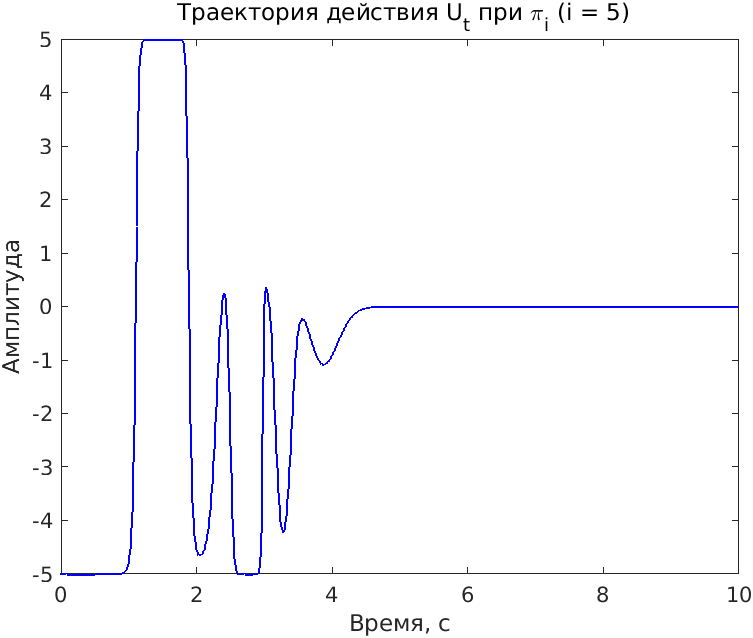
\includegraphics[width=0.9\linewidth]{my_folder/figure/pendul/action.png}\\ \textit{a}}
	\end{minipage}
	\hfill
	\begin{minipage}[h]{0.49\linewidth}
		\center{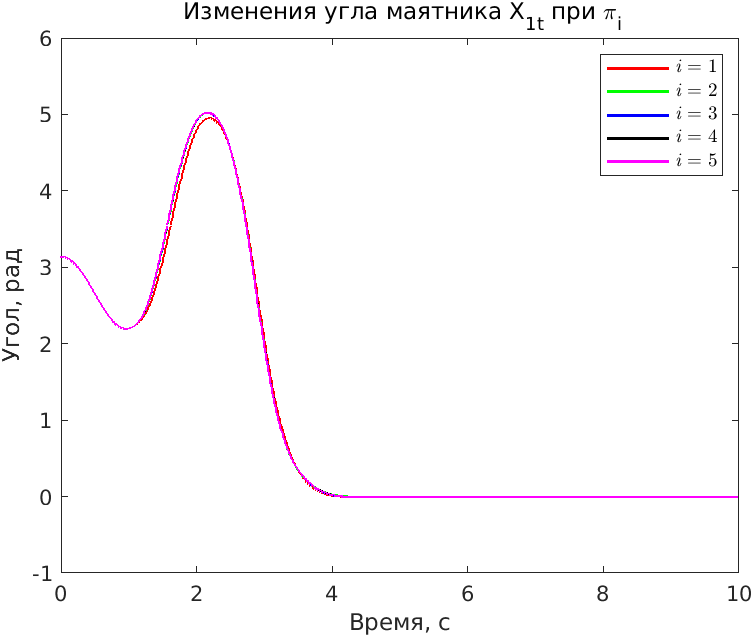
\includegraphics[width=0.9\linewidth]{my_folder/figure/pendul/traj_.png}\\ \textit{б}}
	\end{minipage}
	\hfill
	\begin{minipage}[h]{0.49\linewidth}
		\center{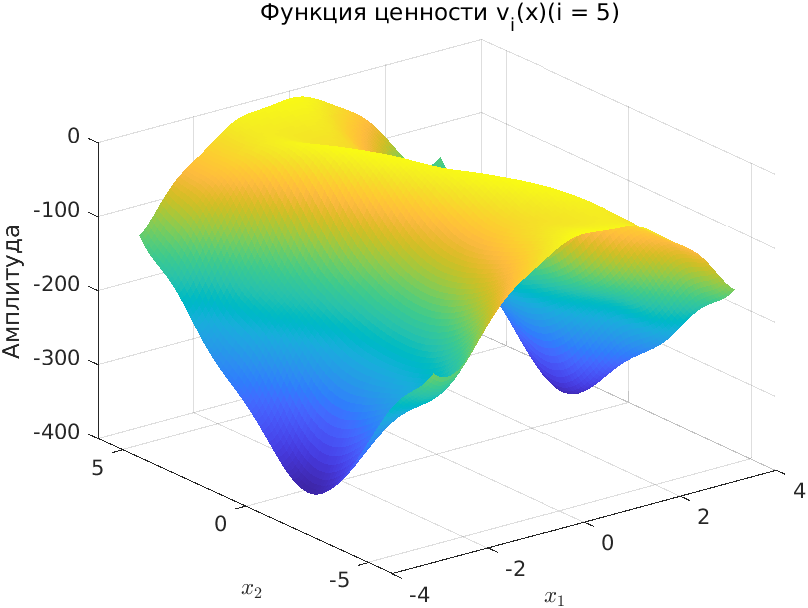
\includegraphics[width=0.9\linewidth]{my_folder/figure/pendul/val_fun.png}\\ \textit{в}}
	\end{minipage}
	\hfill
	\begin{minipage}[h]{0.49\linewidth}
		\center{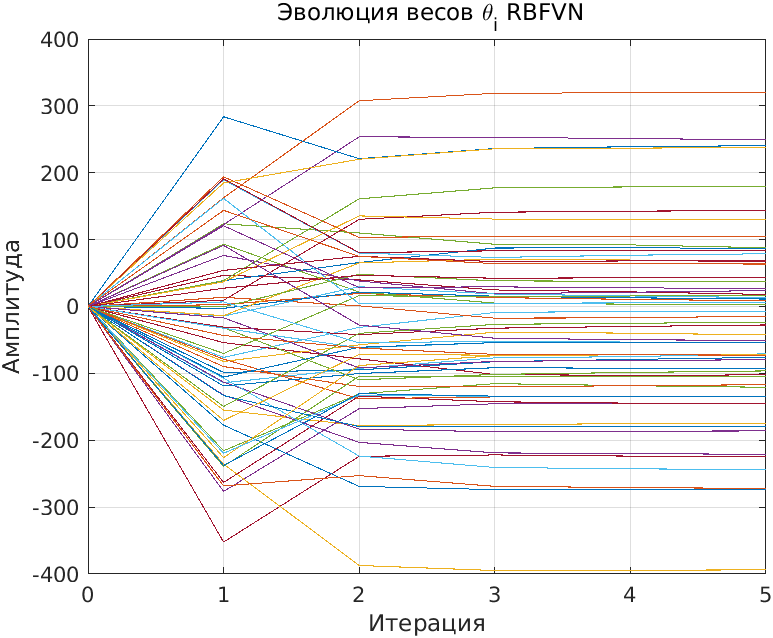
\includegraphics[width=0.85\linewidth]{my_folder/figure/pendul/w.png}\\ \textit{г}}
	\end{minipage}
	\caption{Применение алгоритма DPI для задачи управления обратным маятником; \textit{a} -- управляющее воздействие; \textit{б} -- изменение угла наклона маятника; \textit{в} -- изменение функционала качества; \textit{г} -- график изменения весов}
	\label{fig:pend-ch3}
\end{figure}

%
\section{Управление производством пенициллина}\label{ch3:sec2}
%
Модель биореактора описывает поведение двух видов, которые соревнуются за один субстрат. Реализация систем автоматизации для биореакторов ограничена сложностью синтеза регулятора для систем с большим количеством переменных. Так же автоматизация таких систем ограничена сложностью описания внешних воздействий (например учет воздействия кислорода и углекислого газа на систему), поэтому возникает интерес реализации оптимально-адаптивных регуляторов для таких систем.

В качестве примера рассмотрена модель производства пенициллина  периодического действия \cite{bajpai1980mechanistic}.
Модель была основана на следующих предположениях: 1) рост клеток ограничен субстратом (глюкозой) и кислородом, 2) вся биомасса способна расти и синтезировать пенициллин, 3) образование продукта подавляется субстратом, и 4) требования к техническому обслуживанию постоянны \cite{patnaik2001penicillin}. Модель системы описывается системой однородных дифференциальных уравнений:
%
\begin{equation}\label{eq:penicilin}
\begin{split}
\dot{X} &=\mu(S)X-\frac{u_{\text{inp}}}{V}X,\\
\dot{S} &=-\frac{\mu(S)X}{Y_{\text{x}}}-\frac{vX}{Y_{\text{p}}}+\frac{u_{\text{inp}}}{V}(S_{\text{in}}-S),\\
\dot{P} &=vX-\frac{u_{\text{inp}}}{V}P,\\
\dot{V} &=u_{\text{inp}},\\
\end{split}
\end{equation}
где удельная скорость роста продукта:
\begin{align*}
	\mu(S)&=\frac{\mu_m S}{K_{\text{m}}+S+(S^2/K_{\text{i}})},
\end{align*}
где $X$ -- концентрация биомассы (г/л), $S$ -- концентрация субстрата (г/л), $P$ -- концентрация продукта (г/л), $V$ -- объем биомассы в биореакторе. Управляющим входом является $u$ -- скорость подачи субстрата (г/(л ч)). Параметры модели представлены в \taref{table:penicilin-ch3}
%
\begin{table}[h!]
	\centering
	\small
	\caption{Параметры модели производства пенициллина}
	\begin{tabular}{|p{50pt}|p{190pt}|p{50pt}|p{110pt}|}
		\hline
		
		Параметр  & Описание параметра  & Величина  & Единица измерения  \\
		\hline
		$S_{in}$ & концентрация субстрата в корме & 0.2 & л / (г/л)\\
		\hline
		$Y_x$ & доходность биомассы на единицу массы субстрата & 0.2 & л / (г / ммоль O2)\\
		\hline
		$Y_p$ & доходность продукта на единицу массы субстрата & 1.2 & л /((г / ммоль O2)\\
		\hline
		$\mu_m$& максимальная удельная скорость продукта d &0.02& 1/ч\\
		\hline
		$v$& удельная скорость роста биомассы & 0.004 & 1/ч\\
		\hline
		$K_m$ & константа Моно  & 0.05 & г/л \\
		\hline
		$K_i$ & константа ингибирования  & 5.0 & г/л \\
		\hline
	\end{tabular}
	\label{table:penicilin-ch3}
\end{table}

Цель управления -- получение максимальной концентрации продукта $P$. Задача оптимального управления может быть сформулирована следующим образом:
%
\begin{equation}
\label{f:optimal_task}
\begin{split}
J &= \min_{u, t_f}(\int^{t_f}_0 P(\tau) d\tau) \\
\mathbf{x} &= [X\ S\ P \ V], \space \mathbf{x}(0) = [1.0 \ 0.5 \ 0.01 \ 120.0]^T\\
\dot{\mathbf{x}} &= f(\mathbf{x},u) \\
0 &\le u \le 0.2,\ \  0 \le X\le 3.7, \ \ 0 \le P\le 3.0 \\
0 &\le V \le 125,\ \ S \ge 0 \\
\end{split}
\end{equation}

Для данного объекта управления было реализовано три типа регулятора: оптимальный регулятор, полученный численными методами, регулятор онлайн-оптимизации MPC и регулятор на основе обучения с подкреплением -- Глубокие детерминированные градиенты политики (англ. Deep Deterministic Policy Gradient, DDPG). Используя пакетный модуль OpenOCL, реализованный на языке MATLAB найдено численное решение оптимального управления для модели производства пенициллина. При разработке системы управления методом RL функция награды имела следующий вид: $r = lg(P_k/P_{k-1}) - 50*[X>3.7]-50*[P>3.0]-50*[V>125]$. Результаты моделирования представлены на \firef{fig:bio-ch3}
%
\begin{figure}[ht!]  
	\centering 
	\begin{minipage}[h]{0.49\linewidth}
		\center{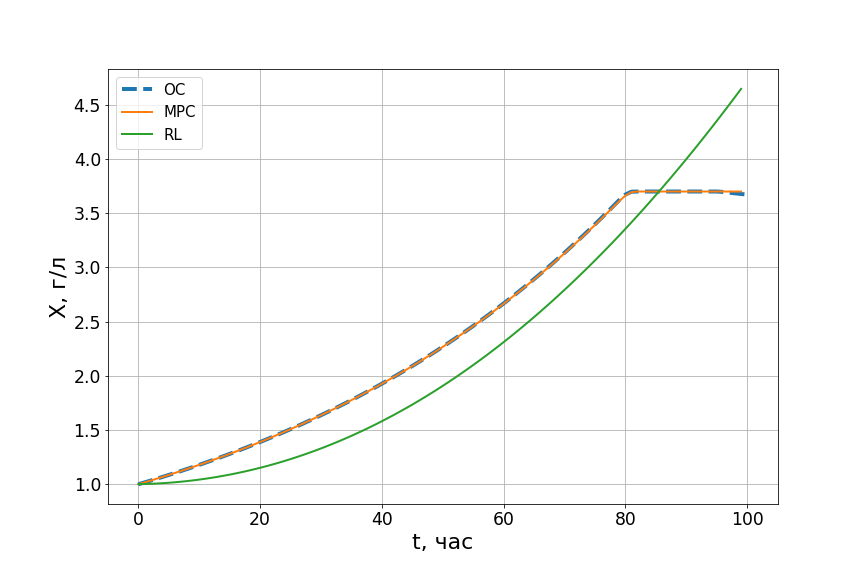
\includegraphics[width=1\linewidth]{my_folder/figure/figure_penicillin/x_MPC_RL.png}\\ \textit{a}}
	\end{minipage}
	\hfill
	\begin{minipage}[h]{0.49\linewidth}
		\center{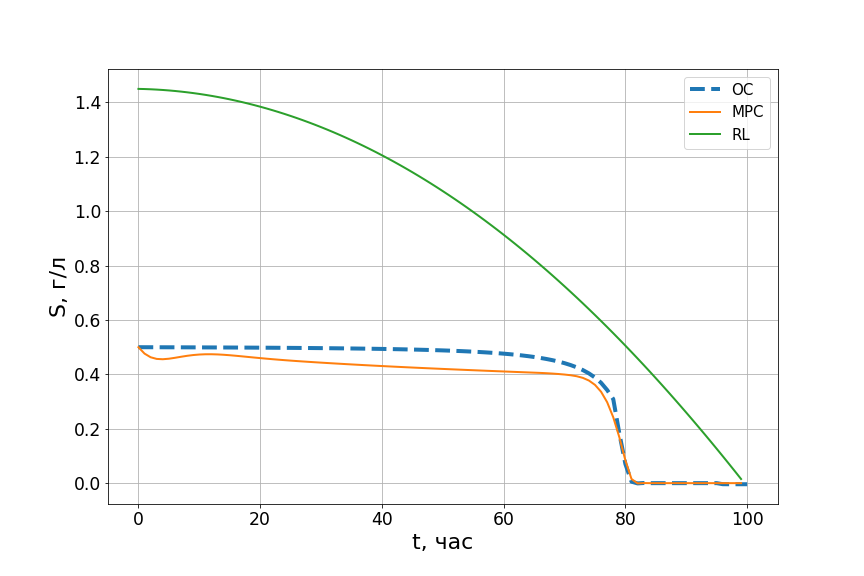
\includegraphics[width=1\linewidth]{my_folder/figure/figure_penicillin/s_MPC_RL.png}\\ \textit{б}}
	\end{minipage}
	\hfill
	\begin{minipage}[h]{0.49\linewidth}
		\center{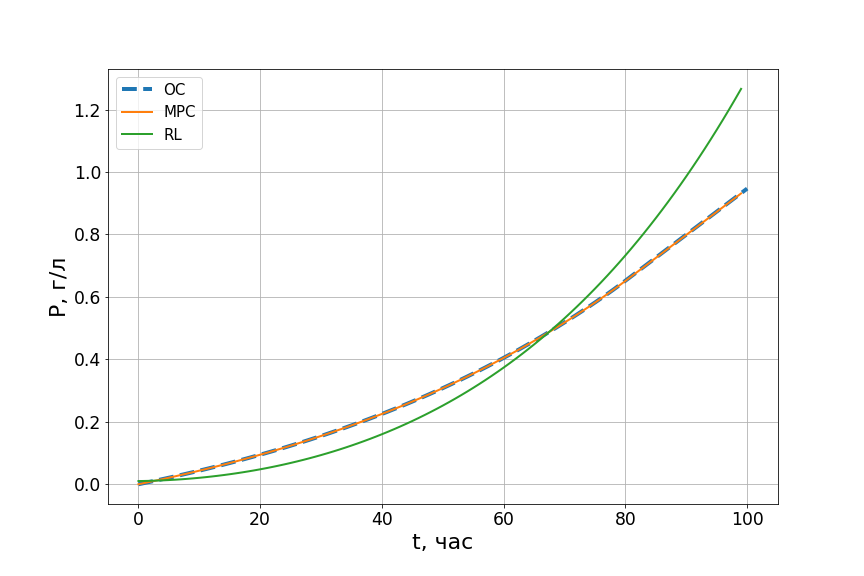
\includegraphics[width=1\linewidth]{my_folder/figure/figure_penicillin/p_MPC_RL.png}\\ \textit{в}}
	\end{minipage}
	\hfill
	\begin{minipage}[h]{0.49\linewidth}
		\center{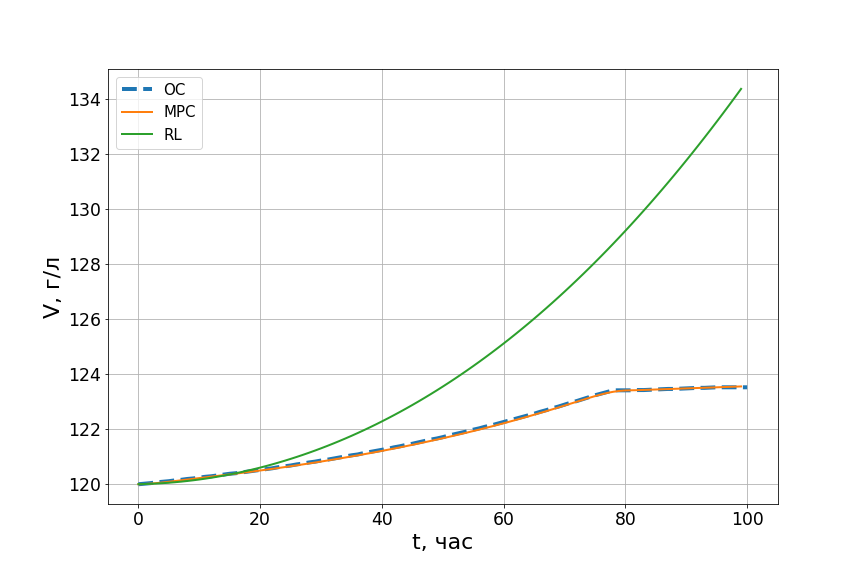
\includegraphics[width=1\linewidth]{my_folder/figure/figure_penicillin/v_MPC_RL.png}\\ \textit{г}}
	\end{minipage}
	\caption{Моделирование управления производства пеницилина: \textit{а} -- изменения концентрации биомассы, \textit{б} -- изменения концентрации субстрата, \textit{в} -- изменения концентрации продукта, \textit{г} -- изменения заполненного объема в биореакторе}
		\label{fig:bio-ch3}
	\end{figure}
%

Для данного процесса важным критерием качества является конечное значение концентрации пенициллина в реакторе $P$. Различие траекторий управляющих воздействий \firef{fig:u_penicillin-ch3} обосновывается не удовлетворительным выбором функции награды, которое предполагается составлять вместе с экспертом. 
\begin{figure}[ht!]
	\center{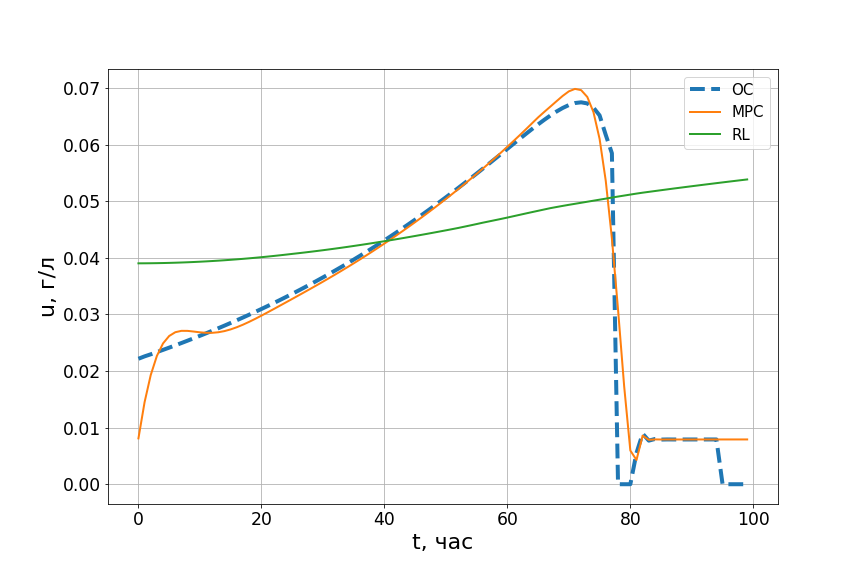
\includegraphics[width=0.5\linewidth]{my_folder/figure/figure_penicillin/u_MPC_RL.png}}
	\caption{Управляющее воздействие, а именно скорость подачи субстрата в реактор}
	\label{fig:u_penicillin-ch3}
\end{figure}


\section{Управление ростом опухоли}\label{ch3:sec2}
%
Рак -- это общее название группы заболеваний, которые включают повторяющееся и неконтролируемое деление и распространение аномальных клеток. Эти аномальные ткани называются опухолями. Ранняя диагностика и эффективное лечение повышают выживаемость больных. Оптимальный график лечения и доза лекарства варьируются в зависимости от стадии опухоли, веса пациента, уровней лейкоцитов (иммунных клеток), сопутствующего заболевания и возраста пациента. Таким образом, правильное планирование и персонализация химиотерапевтического лечения жизненно важны для снижения уровня смертности. 
Чтобы вычислить оптимальную политику управления и вознаграждение, требуется математическая модель, которая показывает воздействие химиотерапевтического препарата в динамике. Реалистичная модель должна учитывать рост опухоли, реакцию иммунной системы человека на рост опухоли и влияние химиотерапевтического лечения на иммунные клетки, нормальные клетки и рост опухоли.

Одна из основных проблем, связанных с изучением рака как динамической системы, состоит в том, что как и любое другое заболевание, известен своей сложной, нелинейной и неопределенной механикой действия. Следовательно, математические модели в дифференциальных уравнениях не в состоянии учесть все вариации в динамике пациента, поэтому поставлена задача разработки регулятора на основе обучения с подкреплением.

В работе \cite{kuznetsov1994nonlinear} представлена фармакологическая модель химиотерапии рака, заданная нелинейной системой из 4-х детерминированных однородных дифференциальных уравнений:
\begin{equation}
\begin{split}
\dot T &= r_1T(1-b_1T) - c_2IT-c_3TN-a_2(1-e^{-M})T,\\
\dot N &= r_2N(1-b_2N) - c_4TN-a_3(1-e^{-M})N, \\
\dot I &= s + \frac{\rho IT}{\alpha + T} - c_1IT - d_1I - a_1(1-e^{-M})I, \\
\dot M &= u(t) - d_2M
\end{split}
\end{equation}
где $T(t)$ -- концентрация раковых клеток,  $N(t)$ -- концентрация нормальных клеток $I(t)$ -- концентрация иммунных клеток в крови (лейкоцитов), и $M(t)$ -- концентрация химиотерапевтического препарата в крови. Управляющее воздействие $u(t)$ соответствует скорости ввода препарата (мг/(л день)). Параметры модели представлены в \taref{table:plana-ch3}.
%
\begin{table}[h!]
	\centering
	\small
	\caption{Параметры модели опухоли}
	\begin{tabular}{|p{45pt}|p{210pt}|p{50pt}|p{100pt}|}
		\hline
		Параметр  & Описание параметра  & Величина  & Единица измерения  \\
		\hline
		$a_1$ & скорость фракционного уничтожения иммунных клеток & 0.2 & л / (мг день)\\
		\hline
		$a_2$ & скорость фракционного уничтожения опухолевых клеток & 0.3 & л / (мг день)\\
		\hline
		$a_3$ & скорость фракционного уничтожения нормальных клеток & 0.1 & л / (мг день)\\
		\hline
		$b_1$ & взаимная несущая способность опухолевых клеток & 1 & 1 / клетка\\
		\hline
		$b_2$ & взаимная несущая способность нормальных клеток & 1 & 1 / клетка\\
		\hline
		$c_1$ & срок конкуренции иммунных клеток (конкуренция между опухолевыми и иммунными клетками) & 1 & 1 / (клетка день)\\
		\hline
		$c_2$ & срок конкуренции опухолевых клеток (конкуренция между опухолевыми и иммунными)& 0.5 & 1 / (клетка день)\\
		\hline
		$c_3$ & срок конкуренции опухолевых клеток (конкуренция между нормальными и опухолевыми) & 1 & 1 / (клетка день)\\
		\hline
		$c_4$ & срок конкуренции нормальных клеток конкуренция между нормальными и опухолевыми) & 1 & 1 / (клетка день)\\
		\hline
		$d_1$ & Темп гибели иммунных клеток & 0.2 & 1 / день\\
		\hline
		$d_2$ & Скорость распада вводимого медицинского препарата & 1 & 1 / день\\
		\hline
		$r_1$ & Скорости роста опухолевых клеток (на единицу) & 1.5 & 1 / день\\
		\hline
		$r_2$ & Скорости роста нормальных клеток (на единицу) & 1 & 1 / день\\
		\hline
		$s$ & Скорость притока иммунных клеток & 0.33 & клетка / день\\
		\hline
		$\alpha$ & Скорость иммунного порога (порогового входа) & 0.3 & клетка \\
		\hline
		$\rho$ & Скорость иммунного ответа & 0.01 & 1 / день\\
		\hline
		
	\end{tabular}
	\label{table:plana-ch3}
\end{table}
%

При разработке схемы лечения важно оптимизировать количество используемого лекарства, чтобы регулировать побочные эффекты химиотерапии, поскольку часто иммунная система пациента ослабевает и становится склонной к опасным для жизни инфекциям, что снижает ее способность искоренить рак. В литературе рассматривается два случая: основной и подготовительный -- несколько нереалистичный случай, в котором цель состоит в том, чтобы искоренить рак независимо от состояния популяции остальных клеток. В обоих случаях начальное условие было одинаковым: [0,7 1 1 0] T.

Задача оптимального управления для упрощенного случая, может быть сформулирована следующим образом:
%
\begin{equation*}
\label{f:optimal_task}
\begin{split}
J &= \min_{u, t_f}(\int^{t_f}_0 T(\tau) d\tau) \\
\mathbf{x} &= [T\ N\ I \ M], \ \ \mathbf{x}(0) = [0.7 \ 1 \ 1 \ 0]^T\\
\dot{\mathbf{x}} &= f(\mathbf{x},u) \\
0 &\le u \le 10 
\end{split}
\end{equation*}

Тогда как такую задачу в терминах RL, опираясь на гипотезу о награде сформировать в виде функции вознаграждения: $R = -dt \cdot T$. В этом случае dt включено в вознаграждение только для того, чтобы упростить сравнение с функционалом качества, приведенного в постановке задачи оптимального управления.
Решением такого случае станет подача максимального значения управляющего воздействия на вход системы. 

Рассмотрим реальный случай. Чтобы гарантировать безопасность пациента во время лечения, к постановке (\ref{f:optimal_task}) добавлены дополнительные ограничения состояния. В частности $N (t) \ge 0,4$ и $I (t) \ge 0,4$
Для задачи RL награда будет равна:
\begin{equation*}
	R = dt \cdot (-T - 0.5 \cdot [N < 0.4] - 0.5 \cdot [I < 0.4])
\end{equation*}


На рисунке приведены графики моделирования при оптимальном управления, регулирования на основе MPC и регулятора на основе алгоритма обучения с подкреплением расширения глубоких детерминированных градиентов политики (англ. Twin Delayed Deep Deterministic Policy Gradients, TD3). Результаты моделирования при регулировании представленны на \firef{fig:tumor-ch3} и \firef{fig:u-ch3}.

\begin{figure}[ht!]  
	\centering 
	\begin{minipage}[h]{0.49\linewidth}
		\center{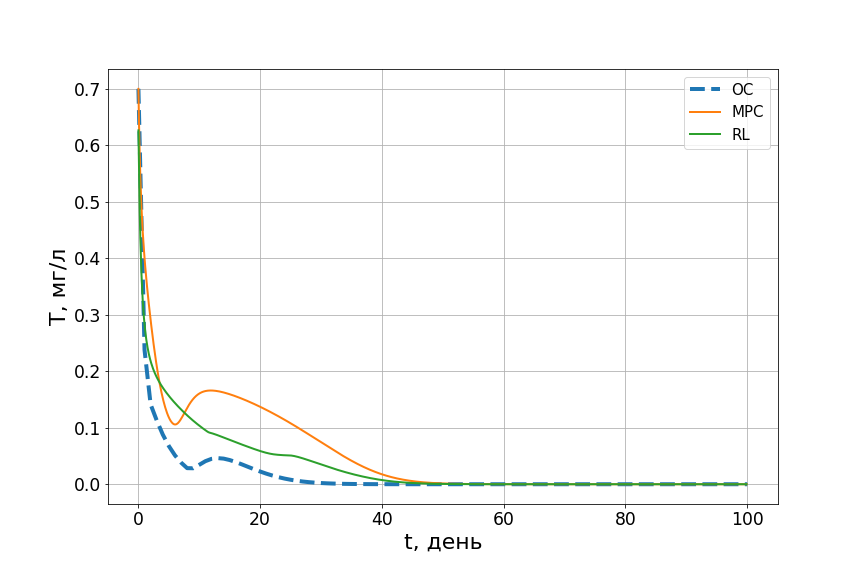
\includegraphics[width=1\linewidth]{my_folder/figure/tumor/T_MPC_RL.png}\\ \textit{a}}
	\end{minipage}
	\hfill
	\begin{minipage}[h]{0.49\linewidth}
		\center{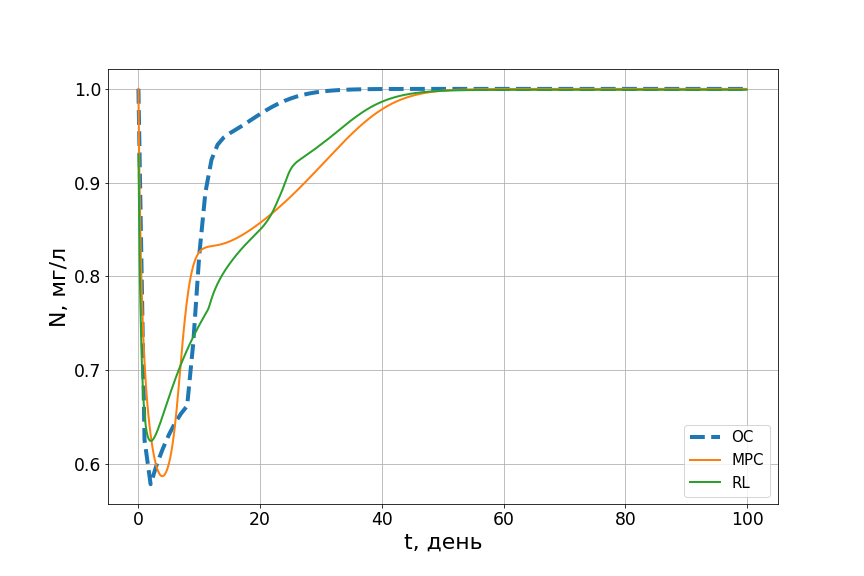
\includegraphics[width=1\linewidth]{my_folder/figure/tumor/N_MPC_RL.png}\\ \textit{б}}
	\end{minipage}
	\hfill
	\begin{minipage}[h]{0.49\linewidth}
		\center{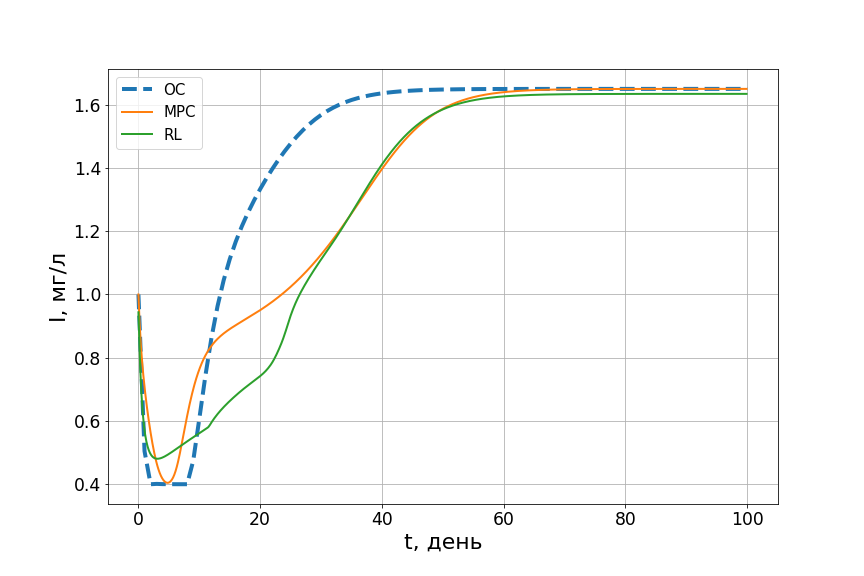
\includegraphics[width=1\linewidth]{my_folder/figure/tumor/I_MPC_RL.png}\\ \textit{в}}
	\end{minipage}
	\hfill
	\begin{minipage}[h]{0.49\linewidth}
		\center{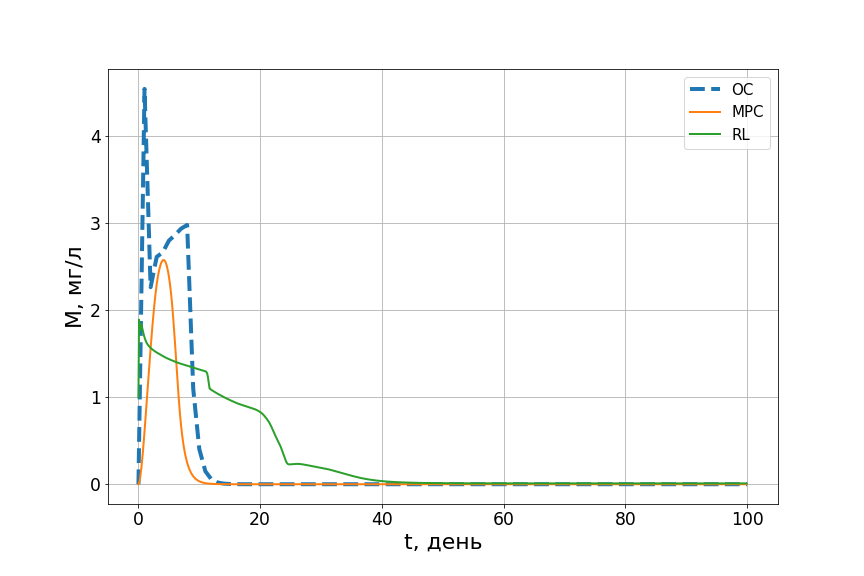
\includegraphics[width=1\linewidth]{my_folder/figure/tumor/M_MPC_RL.png}\\ \textit{г}}
	\end{minipage}
	\caption{Моделирование управления ростом опухоли: \textit{а} -- изменение концентрации раковых клеток, \textit{б} -- изменение концентрации нормальных клеток, \textit{в} -- изменение концентрации иммунных клеток в крови (лейкоцитов), \textit{в} изменение концентрации химиотерапевтического препарата в крови}
	\label{fig:tumor-ch3}
\end{figure}
\begin{figure}[ht!]
	\center{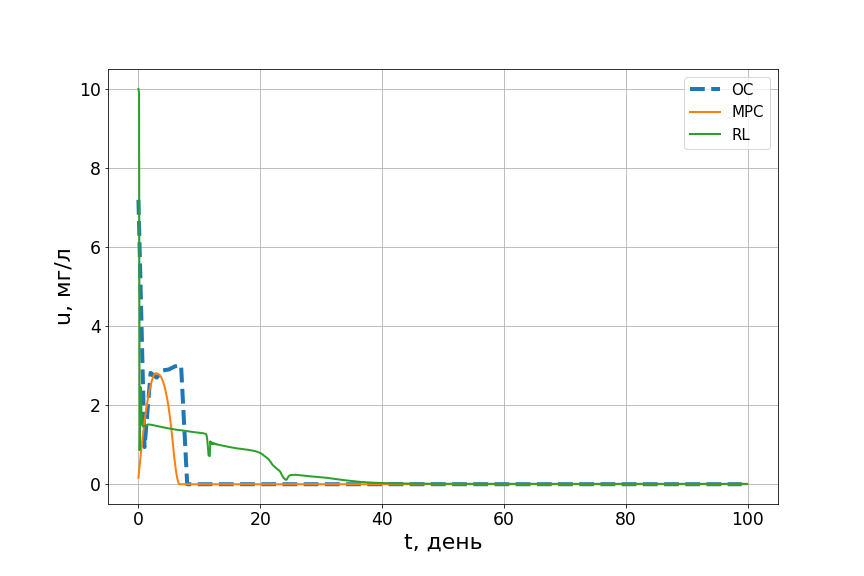
\includegraphics[width=0.65\linewidth]{my_folder/figure/tumor/u_MPC_RL.png}}
	\caption{Управляющее воздействие, представленное скоростью ввода препарата }
	\label{fig:u-ch3}
\end{figure}


Вывод по главе \thechapter. В ходе проведения модельных экспериментов и разработки регуляторов для сложных объектов было установлено:
\begin{itemize}
	
	\item Эксперимент по разработке регулятора для управления производством пенициллина показал, что качество работы безмодельных алгоритмов обучения с подкреплением сильно зависит от дизайна  функционала качества, что только подтверждает указанную проблему в главе 2;
	\item Для задачи управления перевернутым маятников регулятор на основе модельного алгоритма обучения с подкреплением учел ограничения, которые были указаны при разработке функционала качества; 
	\item Регулятор на основе обучения с подкрепления для задачи управления роста опухоли показал такие же высокие качества управления как оптимальный регулятор и регулятор на основе онлайн оптимизации MPC;
	\item Проведенные эксперименты подтверждают применимость методов обучения с подкреплением для задач управления сложными объектами;
\end{itemize}

\newpage
%% Вспомогательные команды - Additional commands
%
%\newpage % принудительное начало с новой страницы, использовать только в конце раздела
%\clearpage % осуществляется пакетом <<placeins>> в пределах секций
%\newpage\leavevmode\thispagestyle{empty}\newpage % 100 % начало новой страницы